\documentclass[a4paper, 12pt]{article}
%%%%%%%%%%%%%%%%%%%%%%%%%%%%%%%%%%%%%%%%%%%%%%%%%%%%%%%%%%%%%%%%%%%%%%%%%%%%%%%
%                                Basic Packages                               %
%%%%%%%%%%%%%%%%%%%%%%%%%%%%%%%%%%%%%%%%%%%%%%%%%%%%%%%%%%%%%%%%%%%%%%%%%%%%%%%

% Gives us multiple colors.
\usepackage[usenames,dvipsnames,pdftex]{xcolor}
% Lets us style link colors.
\usepackage{hyperref}
% Lets us import images and graphics.
\usepackage{graphicx}
% Lets us use figures in floating environments.
\usepackage{float}
% Lets us create multiple columns.
\usepackage{multicol}
% Gives us better math syntax.
\usepackage{amsmath,amsfonts,mathtools,amsthm,amssymb}
% Lets us strikethrough text.
\usepackage{cancel}
% Lets us edit the caption of a figure.
\usepackage{caption}
% Lets us import pdf directly in our tex code.
\usepackage{pdfpages}
% Lets us do algorithm stuff.
\usepackage[ruled,vlined,linesnumbered]{algorithm2e}
% Use a smiley face for our qed symbol.
\usepackage{tikzsymbols}
% \usepackage{fullpage} %%smaller margins
\usepackage[shortlabels]{enumitem}

\setlist[enumerate]{font={\bfseries}} % global settings, for all lists

\usepackage{setspace}
\usepackage[margin=1in, headsep=12pt]{geometry}
\usepackage{wrapfig}
\usepackage{listings}
\usepackage{parskip}

\definecolor{codegreen}{rgb}{0,0.6,0}
\definecolor{codegray}{rgb}{0.5,0.5,0.5}
\definecolor{codepurple}{rgb}{0.58,0,0.82}
\definecolor{backcolour}{rgb}{0.95,0.95,0.95}

\lstdefinestyle{mystyle}{
    backgroundcolor=\color{backcolour},   
    commentstyle=\color{codegreen},
    keywordstyle=\color{magenta},
    numberstyle=\tiny\color{codegray},
    stringstyle=\color{codepurple},
    basicstyle=\ttfamily\footnotesize,
    breakatwhitespace=false,         
    breaklines=true,                 
    captionpos=b,                    
    keepspaces=true,                 
    numbers=left,                    
    numbersep=5pt,                  
    showspaces=false,                
    showstringspaces=false,
    showtabs=false,                  
    tabsize=2,
    numbers=none
}

\lstset{style=mystyle}
\def\class{article}


%%%%%%%%%%%%%%%%%%%%%%%%%%%%%%%%%%%%%%%%%%%%%%%%%%%%%%%%%%%%%%%%%%%%%%%%%%%%%%%
%                                Basic Settings                               %
%%%%%%%%%%%%%%%%%%%%%%%%%%%%%%%%%%%%%%%%%%%%%%%%%%%%%%%%%%%%%%%%%%%%%%%%%%%%%%%

%%%%%%%%%%%%%
%  Symbols  %
%%%%%%%%%%%%%

\let\implies\Rightarrow
\let\impliedby\Leftarrow
\let\iff\Leftrightarrow
\let\epsilon\varepsilon
%%%%%%%%%%%%
%  Tables  %
%%%%%%%%%%%%

\setlength{\tabcolsep}{5pt}
\renewcommand\arraystretch{1.5}

%%%%%%%%%%%%%%
%  SI Unitx  %
%%%%%%%%%%%%%%

\usepackage{siunitx}
\sisetup{locale = FR}

%%%%%%%%%%
%  TikZ  %
%%%%%%%%%%

\usepackage[framemethod=TikZ]{mdframed}
\usepackage{tikz}
\usepackage{tikz-cd}
\usepackage{tikzsymbols}

\usetikzlibrary{intersections, angles, quotes, calc, positioning}
\usetikzlibrary{arrows.meta}

\tikzset{
    force/.style={thick, {Circle[length=2pt]}-stealth, shorten <=-1pt}
}

%%%%%%%%%%%%%%%
%  PGF Plots  %
%%%%%%%%%%%%%%%

\usepackage{pgfplots}
\pgfplotsset{width=10cm, compat=newest}

%%%%%%%%%%%%%%%%%%%%%%%
%  Center Title Page  %
%%%%%%%%%%%%%%%%%%%%%%%

\usepackage{titling}
\renewcommand\maketitlehooka{\null\mbox{}\vfill}
\renewcommand\maketitlehookd{\vfill\null}

%%%%%%%%%%%%%%%%%%%%%%%%%%%%%%%%%%%%%%%%%%%%%%%%%%%%%%%
%  Create a grey background in the middle of the PDF  %
%%%%%%%%%%%%%%%%%%%%%%%%%%%%%%%%%%%%%%%%%%%%%%%%%%%%%%%

\usepackage{eso-pic}
\newcommand\definegraybackground{
    \definecolor{reallylightgray}{HTML}{FAFAFA}
    \AddToShipoutPicture{
        \ifthenelse{\isodd{\thepage}}{
            \AtPageLowerLeft{
                \put(\LenToUnit{\dimexpr\paperwidth-222pt},0){
                    \color{reallylightgray}\rule{222pt}{297mm}
                }
            }
        }
        {
            \AtPageLowerLeft{
                \color{reallylightgray}\rule{222pt}{297mm}
            }
        }
    }
}

%%%%%%%%%%%%%%%%%%%%%%%%
%  Modify Links Color  %
%%%%%%%%%%%%%%%%%%%%%%%%

\hypersetup{
    % Enable highlighting links.
    colorlinks,
    % Change the color of links to blue.
    urlcolor=blue,
    % Change the color of citations to black.
    citecolor={black},
    % Change the color of url's to blue with some black.
    linkcolor={blue!80!black}
}

%%%%%%%%%%%%%%%%%%
% Fix WrapFigure %
%%%%%%%%%%%%%%%%%%

\newcommand{\wrapfill}{\par\ifnum\value{WF@wrappedlines}>0
        \parskip=0pt
        \addtocounter{WF@wrappedlines}{-1}%
        \null\vspace{\arabic{WF@wrappedlines}\baselineskip}%
        \WFclear
    \fi}

%%%%%%%%%%%%%%%%%
% Multi Columns %
%%%%%%%%%%%%%%%%%

\let\multicolmulticols\multicols
\let\endmulticolmulticols\endmulticols

\RenewDocumentEnvironment{multicols}{mO{}}
{%
    \ifnum#1=1
        #2%
    \else % More than 1 column
        \multicolmulticols{#1}[#2]
    \fi
}
{%
    \ifnum#1=1
    \else % More than 1 column
        \endmulticolmulticols
    \fi
}

\newlength{\thickarrayrulewidth}
\setlength{\thickarrayrulewidth}{5\arrayrulewidth}


%%%%%%%%%%%%%%%%%%%%%%%%%%%%%%%%%%%%%%%%%%%%%%%%%%%%%%%%%%%%%%%%%%%%%%%%%%%%%%%
%                           School Specific Commands                          %
%%%%%%%%%%%%%%%%%%%%%%%%%%%%%%%%%%%%%%%%%%%%%%%%%%%%%%%%%%%%%%%%%%%%%%%%%%%%%%%

%%%%%%%%%%%%%%%%%%%%%%%%%%%
%  Initiate New Counters  %
%%%%%%%%%%%%%%%%%%%%%%%%%%%

\newcounter{lecturecounter}

%%%%%%%%%%%%%%%%%%%%%%%%%%
%  Helpful New Commands  %
%%%%%%%%%%%%%%%%%%%%%%%%%%

\makeatletter

\newcommand\resetcounters{
    % Reset the counters for subsection, subsubsection and the definition
    % all the custom environments.
    \setcounter{subsection}{0}
    \setcounter{subsubsection}{0}
    \setcounter{definition0}{0}
    \setcounter{paragraph}{0}
    \setcounter{theorem}{0}
    \setcounter{claim}{0}
    \setcounter{corollary}{0}
    \setcounter{proposition}{0}
    \setcounter{lemma}{0}
    \setcounter{exercise}{0}
    \setcounter{problem}{0}
    
    \setcounter{subparagraph}{0}
    % \@ifclasswith\class{nocolor}{
    %     \setcounter{definition}{0}
    % }{}
}

%%%%%%%%%%%%%%%%%%%%%
%  Lecture Command  %
%%%%%%%%%%%%%%%%%%%%%

\usepackage{xifthen}

% EXAMPLE:
% 1. \lecture{Oct 17 2022 Mon (08:46:48)}{Lecture Title}
% 2. \lecture[4]{Oct 17 2022 Mon (08:46:48)}{Lecture Title}
% 3. \lecture{Oct 17 2022 Mon (08:46:48)}{}
% 4. \lecture[4]{Oct 17 2022 Mon (08:46:48)}{}
% Parameters:
% 1. (Optional) lecture number.
% 2. Time and date of lecture.
% 3. Lecture Title.
\def\@lecture{}
\def\@lectitle{}
\def\@leccount{}
\newcommand\lecture[3]{
    \newpage

    % Check if user passed the lecture title or not.
    \def\@leccount{Lecture #1}
    \ifthenelse{\isempty{#3}}{
        \def\@lecture{Lecture #1}
        \def\@lectitle{Lecture #1}
    }{
        \def\@lecture{Lecture #1: #3}
        \def\@lectitle{#3}
    }

    \setcounter{section}{#1}
    \renewcommand\thesubsection{#1.\arabic{subsection}}
    
    \phantomsection
    \addcontentsline{toc}{section}{\@lecture}
    \resetcounters

    \begin{mdframed}
        \begin{center}
            \Large \textbf{\@leccount}
            
            \vspace*{0.2cm}
            
            \large \@lectitle
            
            
            \vspace*{0.2cm}

            \normalsize #2
        \end{center}
    \end{mdframed}

}

%%%%%%%%%%%%%%%%%%%%
%  Import Figures  %
%%%%%%%%%%%%%%%%%%%%

\usepackage{import}
\pdfminorversion=7

% EXAMPLE:
% 1. \incfig{limit-graph}
% 2. \incfig[0.4]{limit-graph}
% Parameters:
% 1. The figure name. It should be located in figures/NAME.tex_pdf.
% 2. (Optional) The width of the figure. Example: 0.5, 0.35.
\newcommand\incfig[2][1]{%
    \def\svgwidth{#1\columnwidth}
    \import{./figures/}{#2.pdf_tex}
}

\begingroup\expandafter\expandafter\expandafter\endgroup
\expandafter\ifx\csname pdfsuppresswarningpagegroup\endcsname\relax
\else
    \pdfsuppresswarningpagegroup=1\relax
\fi

%%%%%%%%%%%%%%%%%
% Fancy Headers %
%%%%%%%%%%%%%%%%%

\usepackage{fancyhdr}

% Force a new page.
\newcommand\forcenewpage{\clearpage\mbox{~}\clearpage\newpage}

% This command makes it easier to manage my headers and footers.
\newcommand\createintro{
    % Use roman page numbers (e.g. i, v, vi, x, ...)
    \pagenumbering{roman}

    % Display the page style.
    \maketitle
    % Make the title pagestyle empty, meaning no fancy headers and footers.
    \thispagestyle{empty}
    % Create a newpage.
    \newpage

    % Input the intro.tex page if it exists.
    \IfFileExists{intro.tex}{ % If the intro.tex file exists.
        % Input the intro.tex file.
        \textbf{Course}: MATH 16300: Honors Calculus III

\textbf{Section}: 43

\textbf{Professor}: Minjae Park

\textbf{At}: The University of Chicago

\textbf{Quarter}: Spring 2023

\textbf{Course materials}: Calculus by Spivak (4th Edition), Calculus On Manifolds by Spivak

\vspace{1cm}
\textbf{Disclaimer}: This document will inevitably contain some mistakes, both simple typos and serious logical and mathematical errors. Take what you read with a grain of salt as it is made by an undergraduate student going through the learning process himself. If you do find any error, I would really appreciate it if you can let me know by email at \href{mailto:conghungletran@gmail.com}{conghungletran@gmail.com}.

        % Make the pagestyle fancy for the intro.tex page.
        \pagestyle{fancy}

        % Remove the line for the header.
        \renewcommand\headrulewidth{0pt}

        % Remove all header stuff.
        \fancyhead{}

        % Add stuff for the footer in the center.
        % \fancyfoot[C]{
        %   \textit{For more notes like this, visit
        %   \href{\linktootherpages}{\shortlinkname}}. \\
        %   \vspace{0.1cm}
        %   \hrule
        %   \vspace{0.1cm}
        %   \@author, \\
        %   \term: \academicyear, \\
        %   Last Update: \@date, \\
        %   \faculty
        % }

        \newpage
    }{ % If the intro.tex file doesn't exist.
        % Force a \newpageage.
        % \forcenewpage
        \newpage
    }

    % Remove the center stuff we did above, and replace it with just the page
    % number, which is still in roman numerals.
    \fancyfoot[C]{\thepage}
    % Add the table of contents.
    \tableofcontents
    % Force a new page.
    \newpage

    % Move the page numberings back to arabic, from roman numerals.
    \pagenumbering{arabic}
    % Set the page number to 1.
    \setcounter{page}{1}

    % Add the header line back.
    \renewcommand\headrulewidth{0.4pt}
    % In the top right, add the lecture title.
    \fancyhead[R]{\footnotesize \@lecture}
    % In the top left, add the author name.
    \fancyhead[L]{\footnotesize \@author}
    % In the bottom center, add the page.
    \fancyfoot[C]{\thepage}
    % Add a nice gray background in the middle of all the upcoming pages.
    % \definegraybackground
}

\makeatother


%%%%%%%%%%%%%%%%%%%%%%%%%%%%%%%%%%%%%%%%%%%%%%%%%%%%%%%%%%%%%%%%%%%%%%%%%%%%%%%
%                               Custom Commands                               %
%%%%%%%%%%%%%%%%%%%%%%%%%%%%%%%%%%%%%%%%%%%%%%%%%%%%%%%%%%%%%%%%%%%%%%%%%%%%%%%

%%%%%%%%%%%%
%  Circle  %
%%%%%%%%%%%%

\newcommand*\circled[1]{\tikz[baseline= (char.base)]{
        \node[shape=circle,draw,inner sep=1pt] (char) {#1};}
}

%%%%%%%%%%%%%%%%%%%
%  Todo Commands  %
%%%%%%%%%%%%%%%%%%%

% \usepackage{xargs}
% \usepackage[colorinlistoftodos]{todonotes}

% \makeatletter

% \@ifclasswith\class{working}{
%     \newcommandx\unsure[2][1=]{\todo[linecolor=red,backgroundcolor=red!25,bordercolor=red,#1]{#2}}
%     \newcommandx\change[2][1=]{\todo[linecolor=blue,backgroundcolor=blue!25,bordercolor=blue,#1]{#2}}
%     \newcommandx\info[2][1=]{\todo[linecolor=OliveGreen,backgroundcolor=OliveGreen!25,bordercolor=OliveGreen,#1]{#2}}
%     \newcommandx\improvement[2][1=]{\todo[linecolor=Plum,backgroundcolor=Plum!25,bordercolor=Plum,#1]{#2}}

%     \newcommand\listnotes{
%         \newpage
%         \listoftodos[Notes]
%     }
% }{
%     \newcommandx\unsure[2][1=]{}
%     \newcommandx\change[2][1=]{}
%     \newcommandx\info[2][1=]{}
%     \newcommandx\improvement[2][1=]{}

%     \newcommand\listnotes{}
% }

% \makeatother

%%%%%%%%%%%%%
%  Correct  %
%%%%%%%%%%%%%

% EXAMPLE:
% 1. \correct{INCORRECT}{CORRECT}
% Parameters:
% 1. The incorrect statement.
% 2. The correct statement.
\definecolor{correct}{HTML}{009900}
\newcommand\correct[2]{{\color{red}{#1 }}\ensuremath{\to}{\color{correct}{ #2}}}


%%%%%%%%%%%%%%%%%%%%%%%%%%%%%%%%%%%%%%%%%%%%%%%%%%%%%%%%%%%%%%%%%%%%%%%%%%%%%%%
%                                 Environments                                %
%%%%%%%%%%%%%%%%%%%%%%%%%%%%%%%%%%%%%%%%%%%%%%%%%%%%%%%%%%%%%%%%%%%%%%%%%%%%%%%

\usepackage{varwidth}
\usepackage{thmtools}
\usepackage[most,many,breakable]{tcolorbox}

\tcbuselibrary{theorems,skins,hooks}
\usetikzlibrary{arrows,calc,shadows.blur}

%%%%%%%%%%%%%%%%%%%
%  Define Colors  %
%%%%%%%%%%%%%%%%%%%

% color prototype
% \definecolor{color}{RGB}{45, 111, 177}

% ESSENTIALS: 
\definecolor{myred}{HTML}{c74540}
\definecolor{myblue}{HTML}{072b85}
\definecolor{mygreen}{HTML}{388c46}
\definecolor{myblack}{HTML}{000000}

\colorlet{definition_color}{myred}

\colorlet{theorem_color}{myblue}
\colorlet{lemma_color}{myblue}
\colorlet{prop_color}{myblue}
\colorlet{corollary_color}{myblue}
\colorlet{claim_color}{myblue}

\colorlet{proof_color}{myblack}
\colorlet{example_color}{myblack}
\colorlet{exercise_color}{myblack}

% MISCS: 
%%%%%%%%%%%%%%%%%%%%%%%%%%%%%%%%%%%%%%%%%%%%%%%%%%%%%%%%%
%  Create Environments Styles Based on Given Parameter  %
%%%%%%%%%%%%%%%%%%%%%%%%%%%%%%%%%%%%%%%%%%%%%%%%%%%%%%%%%

% \mdfsetup{skipabove=1em,skipbelow=0em}

%%%%%%%%%%%%%%%%%%%%%%
%  Helpful Commands  %
%%%%%%%%%%%%%%%%%%%%%%

% EXAMPLE:
% 1. \createnewtheoremstyle{thmdefinitionbox}{}{}
% 2. \createnewtheoremstyle{thmtheorembox}{}{}
% 3. \createnewtheoremstyle{thmproofbox}{qed=\qedsymbol}{
%       rightline=false, topline=false, bottomline=false
%    }
% Parameters:
% 1. Theorem name.
% 2. Any extra parameters to pass directly to declaretheoremstyle.
% 3. Any extra parameters to pass directly to mdframed.
\newcommand\createnewtheoremstyle[3]{
    \declaretheoremstyle[
        headfont=\bfseries\sffamily, bodyfont=\normalfont, #2,
        mdframed={
                #3,
            },
    ]{#1}
}

% EXAMPLE:
% 1. \createnewcoloredtheoremstyle{thmdefinitionbox}{definition}{}{}
% 2. \createnewcoloredtheoremstyle{thmexamplebox}{example}{}{
%       rightline=true, leftline=true, topline=true, bottomline=true
%     }
% 3. \createnewcoloredtheoremstyle{thmproofbox}{proof}{qed=\qedsymbol}{backgroundcolor=white}
% Parameters:
% 1. Theorem name.
% 2. Color of theorem.
% 3. Any extra parameters to pass directly to declaretheoremstyle.
% 4. Any extra parameters to pass directly to mdframed.

% change backgroundcolor to #2!5 if user wants a colored backdrop to theorem environments. It's a cool color theme, but there's too much going on in the page.
\newcommand\createnewcoloredtheoremstyle[4]{
    \declaretheoremstyle[
        headfont=\bfseries\sffamily\color{#2},
        bodyfont=\normalfont,
        headpunct=,
        headformat = \NAME~\NUMBER\NOTE \hfill\smallskip\linebreak,
        #3,
        mdframed={
                outerlinewidth=0.75pt,
                rightline=false,
                leftline=false,
                topline=false,
                bottomline=false,
                backgroundcolor=white,
                skipabove = 5pt,
                skipbelow = 0pt,
                linecolor=#2,
                innertopmargin = 0pt,
                innerbottommargin = 0pt,
                innerrightmargin = 4pt,
                innerleftmargin= 6pt,
                leftmargin = -6pt,
                #4,
            },
    ]{#1}
}



%%%%%%%%%%%%%%%%%%%%%%%%%%%%%%%%%%%
%  Create the Environment Styles  %
%%%%%%%%%%%%%%%%%%%%%%%%%%%%%%%%%%%

\makeatletter
\@ifclasswith\class{nocolor}{
    % Environments without color.

    % ESSENTIALS:
    \createnewtheoremstyle{thmdefinitionbox}{}{}
    \createnewtheoremstyle{thmtheorembox}{}{}
    \createnewtheoremstyle{thmproofbox}{qed=\qedsymbol}{}
    \createnewtheoremstyle{thmcorollarybox}{}{}
    \createnewtheoremstyle{thmlemmabox}{}{}
    \createnewtheoremstyle{thmclaimbox}{}{}
    \createnewtheoremstyle{thmexamplebox}{}{}

    % MISCS: 
    \createnewtheoremstyle{thmpropbox}{}{}
    \createnewtheoremstyle{thmexercisebox}{}{}
    \createnewtheoremstyle{thmexplanationbox}{}{}
    \createnewtheoremstyle{thmremarkbox}{}{}
    
    % STYLIZED MORE BELOW
    \createnewtheoremstyle{thmquestionbox}{}{}
    \createnewtheoremstyle{thmsolutionbox}{qed=\qedsymbol}{}
}{
    % Environments with color.

    % ESSENTIALS: definition, theorem, proof, corollary, lemma, claim, example
    \createnewcoloredtheoremstyle{thmdefinitionbox}{definition_color}{}{leftline=false}
    \createnewcoloredtheoremstyle{thmtheorembox}{theorem_color}{}{leftline=false}
    \createnewcoloredtheoremstyle{thmproofbox}{proof_color}{qed=\qedsymbol}{}
    \createnewcoloredtheoremstyle{thmcorollarybox}{corollary_color}{}{leftline=false}
    \createnewcoloredtheoremstyle{thmlemmabox}{lemma_color}{}{leftline=false}
    \createnewcoloredtheoremstyle{thmpropbox}{prop_color}{}{leftline=false}
    \createnewcoloredtheoremstyle{thmclaimbox}{claim_color}{}{leftline=false}
    \createnewcoloredtheoremstyle{thmexamplebox}{example_color}{}{}
    \createnewcoloredtheoremstyle{thmexplanationbox}{example_color}{qed=\qedsymbol}{}
    \createnewcoloredtheoremstyle{thmremarkbox}{theorem_color}{}{}

    \createnewcoloredtheoremstyle{thmmiscbox}{black}{}{}

    \createnewcoloredtheoremstyle{thmexercisebox}{exercise_color}{}{}
    \createnewcoloredtheoremstyle{thmproblembox}{theorem_color}{}{leftline=false}
    \createnewcoloredtheoremstyle{thmsolutionbox}{mygreen}{qed=\qedsymbol}{}
}
\makeatother

%%%%%%%%%%%%%%%%%%%%%%%%%%%%%
%  Create the Environments  %
%%%%%%%%%%%%%%%%%%%%%%%%%%%%%
\declaretheorem[numberwithin=section, style=thmdefinitionbox,     name=Definition]{definition}
\declaretheorem[numberwithin=section, style=thmtheorembox,     name=Theorem]{theorem}
\declaretheorem[numbered=no,          style=thmexamplebox,     name=Example]{example}
\declaretheorem[numberwithin=section, style=thmtheorembox,       name=Claim]{claim}
\declaretheorem[numberwithin=section, style=thmcorollarybox,   name=Corollary]{corollary}
\declaretheorem[numberwithin=section, style=thmpropbox,        name=Proposition]{proposition}
\declaretheorem[numberwithin=section, style=thmlemmabox,       name=Lemma]{lemma}
\declaretheorem[numberwithin=section, style=thmexercisebox,    name=Exercise]{exercise}
\declaretheorem[numbered=no,          style=thmproofbox,       name=Proof]{proof0}
\declaretheorem[numbered=no,          style=thmexplanationbox, name=Explanation]{explanation}
\declaretheorem[numbered=no,          style=thmsolutionbox,    name=Solution]{solution}
\declaretheorem[numberwithin=section,          style=thmproblembox,     name=Problem]{problem}
\declaretheorem[numbered=no,          style=thmmiscbox,    name=Intuition]{intuition}
\declaretheorem[numbered=no,          style=thmmiscbox,    name=Goal]{goal}
\declaretheorem[numbered=no,          style=thmmiscbox,    name=Recall]{recall}
\declaretheorem[numbered=no,          style=thmmiscbox,    name=Motivation]{motivation}
\declaretheorem[numbered=no,          style=thmmiscbox,    name=Remark]{remark}
\declaretheorem[numbered=no,          style=thmmiscbox,    name=Observe]{observe}
\declaretheorem[numbered=no,          style=thmmiscbox,    name=Question]{question}


%%%%%%%%%%%%%%%%%%%%%%%%%%%%
%  Edit Proof Environment  %
%%%%%%%%%%%%%%%%%%%%%%%%%%%%

\renewenvironment{proof}[2][\proofname]{
    % \vspace{-12pt}
    \begin{proof0} [#2]
        }{\end{proof0}}

\theoremstyle{definition}

\newtheorem*{notation}{Notation}
\newtheorem*{previouslyseen}{As previously seen}
\newtheorem*{property}{Property}
% \newtheorem*{intuition}{Intuition}
% \newtheorem*{goal}{Goal}
% \newtheorem*{recall}{Recall}
% \newtheorem*{motivation}{Motivation}
% \newtheorem*{remark}{Remark}
% \newtheorem*{observe}{Observe}

\author{Hung C. Le Tran}


%%%% MATH SHORTHANDS %%%%
%% blackboard bold math capitals
\DeclareMathOperator*{\esssup}{ess\,sup}
\DeclareMathOperator*{\Hom}{Hom}
\newcommand{\bbf}{\mathbb{F}}
\newcommand{\bbn}{\mathbb{N}}
\newcommand{\bbq}{\mathbb{Q}}
\newcommand{\bbr}{\mathbb{R}}
\newcommand{\bbz}{\mathbb{Z}}
\newcommand{\bbc}{\mathbb{C}}
\newcommand{\bbk}{\mathbb{K}}
\newcommand{\bbm}{\mathbb{M}}
\newcommand{\bbp}{\mathbb{P}}
\newcommand{\bbe}{\mathbb{E}}

\newcommand{\bfw}{\mathbf{w}}
\newcommand{\bfx}{\mathbf{x}}
\newcommand{\bfX}{\mathbf{X}}
\newcommand{\bfy}{\mathbf{y}}
\newcommand{\bfyhat}{\mathbf{\hat{y}}}

\newcommand{\calb}{\mathcal{B}}
\newcommand{\calf}{\mathcal{F}}
\newcommand{\calt}{\mathcal{T}}
\newcommand{\call}{\mathcal{L}}
\renewcommand{\phi}{\varphi}

% Universal Math Shortcuts
\newcommand{\st}{\hspace*{2pt}\text{s.t.}\hspace*{2pt}}
\newcommand{\pffwd}{\hspace*{2pt}\fbox{\(\Rightarrow\)}\hspace*{10pt}}
\newcommand{\pfbwd}{\hspace*{2pt}\fbox{\(\Leftarrow\)}\hspace*{10pt}}
\newcommand{\contra}{\ensuremath{\Rightarrow\Leftarrow}}
\newcommand{\cvgn}{\xrightarrow{n \to \infty}}
\newcommand{\cvgj}{\xrightarrow{j \to \infty}}

\newcommand{\im}{\mathrm{im}}
\newcommand{\innerproduct}[2]{\langle #1, #2 \rangle}
\newcommand*{\conj}[1]{\overline{#1}}

% https://tex.stackexchange.com/questions/438612/space-between-exists-and-forall
% https://tex.stackexchange.com/questions/22798/nice-looking-empty-set
\let\oldforall\forall
\renewcommand{\forall}{\;\oldforall\; }
\let\oldexist\exists
\renewcommand{\exists}{\;\oldexist\; }
\newcommand\existu{\;\oldexist!\: }
\let\oldemptyset\emptyset
\let\emptyset\varnothing


\renewcommand{\_}[1]{\underline{#1}}
\DeclarePairedDelimiter{\abs}{\lvert}{\rvert}
\DeclarePairedDelimiter{\norm}{\lVert}{\rVert}
\DeclarePairedDelimiter\ceil{\lceil}{\rceil}
\DeclarePairedDelimiter\floor{\lfloor}{\rfloor}
\setlength\parindent{0pt}
\setlength{\headheight}{12.0pt}
\addtolength{\topmargin}{-12.0pt}


% Default skipping, change if you want more spacing
% \thinmuskip=3mu
% \medmuskip=4mu plus 2mu minus 4mu
% \thickmuskip=5mu plus 5mu

% \DeclareMathOperator{\ext}{ext}
% \DeclareMathOperator{\bridge}{bridge}
\title{MATH 20700: Honors Analysis in Rn I \\ \large Problem Set 8}
\date{26 Nov 2023}
\author{Hung Le Tran}
\begin{document}
\maketitle
\setcounter{section}{8}
\textbf{Textbook: Pugh's Real Mathematical Analysis}

\textit{Collaborators: Lucio, Hung Pham, Duc}
\begin{problem} [5.48 \redtext{done}]
Set \[
    f(x, y) = \begin{cases}
        1 - 1/q & \:\text{if}\: x, y \in \bbq \cap [0, 1], y = p/q \\
        1       & \:\text{otherwise}\:
    \end{cases}
\]
Prove that $f$ is RI on $R = [0, 1]^2$, calculate $\underline{F}(y)$ and $\overline{F}(y)$, and prove that $\int_{0}^{1} \underline{F}(y) = \int_{0}^{1} \overline{F}(y) dy = \int_{R} f = 1$.
\end{problem}
\begin{solution}
    \textbf{1.} We first WTS $f$ is RI on $R$, by showing that the set of discontinuities is a zero set in $R$. Recall that \[
        D = \bigcup_{k \in \bbn}D_k
    \]
    where $D_k = \{z \in R: osc_z (f) = \lim_{r \to 0} diam (B_R(z, r)) \geq \frac{1}{k}\}$.

    Fix $k \in \bbn$. Let \begin{align*}
        N_k & = \:\text{set of reduced fractions less than 1 with denominators $\leq 2k$}\: \\
            & = \{ 0 \leq p/q \leq 1 : p, q \in \bbn, gcd(p, q) = 1, q \leq 2k\}            \\
            & = \{0, 1/1, 1/2, 1/3, 2/3, 1/4, 3/4, \ldots, (2k-1)/2k\}                      \\
        E_k & = \{(x, y) \in R: y \in N_k\} = [0, 1] \times N_k
    \end{align*}
    Quickly note that $N_k$ is a finite set, since its number of elements is strictly less than $4k^2$. Therefore $E_k$ is a zero set in $R$, since it is a finite union of 1-dimensional slices.


    We want to show that all points in $R \backslash E_k$ has oscillation less than $1/k$.

    Indeed, take any $(x_0, y_0) \in R \backslash E_k = \{(x, y) \in R: y \not \in N_k\}$. Take $d = \min_{a \in N_k}\{|y_0 - a|\} > 0$.

    Then for $r < d$, the ball $B_R((x_0, y_0), r) \cap E_k = \emptyset$. Take $(x, y)\in B_R((x_0, y_0), r)$, then  \[
        f(x, y) = \begin{cases}
            1 - 1/l & \:\text{if}\: x, y \in \bbq \cap [0, 1]; y = l'/l \:\text{for some}\: l > 2k \:\text{since}\: y \not \in N_k \\
            1       & \:\text{otherwise}\:
        \end{cases}
    \]

    Hence for any $z_1, z_2 \in B_R(z, r)$,
    \begin{align*}
        |f(z_1) - f(z_2)| & \leq |f(z_1) - 1| + |f(z_2) - 1|        \\
                          & < |1 - 1/2k - 1| + |1 - 1/2k - 1| = 1/k
    \end{align*}
    which implies \[
        osc_{(x_0, y_0)}(f) = \lim_{r \to 0} diam(B_R(z, r)) < 1/k
    \]

    Therefore all points in $R \backslash E_k$ has oscillation less than $1/k$, which implies $D_k \subset E_k$, which implies $D_k$ is a zero set.

    $D$ is then a countable union of zero sets, and is therefore a zero set. $f$ is RI as required.

    \textbf{2.} To find $\underline{F}(y)$ and $\overline{F}(y)$, we first have to define $f_y(x)$, which is:
    \[
        f_y(x) = \begin{cases}
            1 - \1_\bbq(x)/q & \:\text{if}\: y = p/q \\
            1                & \:\text{otherwise}\:
        \end{cases}
    \]
    \textbf{Case 1:} $y \in \bbq, y = p/q$.
    \begin{align*}
        \underline{F}(y) & = \underline{\int_{0}^{1}} ( 1 - \1_\bbq(x)/q) dx           \\
                         & = \sup_{P \in \mathcal{P}([0, 1])} L ( 1 - \1_\bbq(x)/q, P)
    \end{align*}
    For any partition $P$ of $[0, 1]$, $m_i = 1- 1/q \forall i$, since the rationals are dense in [0, 1]. Therefore $L( 1 - \1_\bbq(x)/q, P) = 1-1/q \forall P$. Therefore \[
        \underline{F}(y) = 1 - 1/q
    \]

    On the other hand, \begin{align*}
        \overline{F}(y) & = \overline{\int_{0}^{1}} ( 1 - \1_\bbq(x)/q) dx            \\
                        & = \inf_{P \in \mathcal{P}([0, 1])} U ( 1 - \1_\bbq(x)/q, P)
    \end{align*}
    For any partition $P$ of $[0, 1]$, $M_i = 1 \forall i$, since the irrationals are dense in [0, 1]. Therefore $U( 1 - \1_\bbq(x)/q, P) = 1 \forall P$. Therefore \[
        \overline{F}(y) = 1
    \]

    \textbf{Case 2:} $y \not \in \bbq$, so $f_y \equiv 1$. Then it's clear that
    \[
        \overline{F}(y) = \underline{F}(y) = 1
    \]

    In conclusion,
    \[
        \underline{F}(y) = \begin{cases}
            1 - 1/q & \:\text{if}\:  y = p/q \\
            1       & \:\text{otherwise}\:
        \end{cases}
    \]\[
        \overline{F}(y) \equiv 1
    \]

    Since $f$ is RI on $R$, it follows that \[
        \int_{0}^1 \underline{F}(y) = \int_{R} f = \int_{0}^{1} \overline{F}(y) = \int_{0}^1 1 dy = 1
    \]
    as required.
\end{solution}


\begin{problem} [5.49 \redtext{done}]
Using the FTC, give a direct proof of Green's Formulas \[
    - \iint_R f_y dx dy = \int_{\partial R} f dx
\]
and \[
    \iint_R g_x dx dy = \int_{\partial R} g dy
\]
where $R$ is a square in the plane and $f, g: \bbr^2 \to \bbr$ are smooth. (Assume that the edges of the square are parallel to the coordinate axes.)
\end{problem}
\begin{solution}
    Let $R = [a, b] \times [c, d]$.
    \begin{center}
    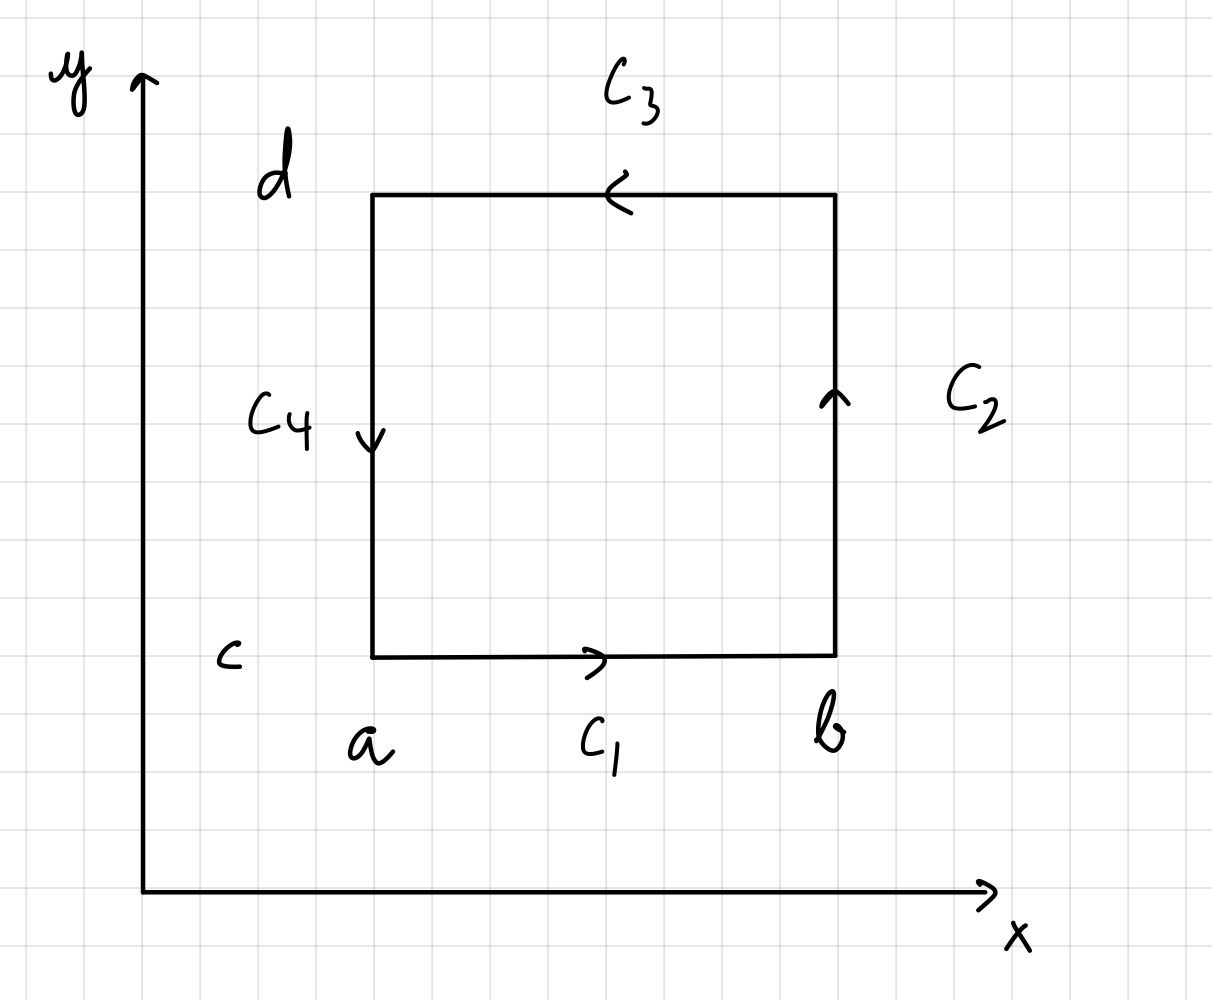
\includegraphics[width=8cm]{./figures/8.2.1.jpeg}
    \end{center}

    Then \begin{align*}
    - \iint_R f_y dx dy &= -\int_{a}^b \int_{c}^{d} f_y dy dx \\
    &= - \int_{a}^{b} f(x, y=d) - f(x, y=c) dx \\
    &= \int_{a}^{b} f(x, y= c) dx - \int_{a}^{b} f(x, y=d) dx \\
    &= \int_{C_1} f dx + \int_{C_3} f dx \\
    &= \int_{\partial R} f dx
    \end{align*}
    since on $C_2$ and $C_4$, $x$ stays unchanged so $\int_{C_2} f dx = \int_{C_4} f dx = 0$.
    Similarly, \begin{align*}
    \iint_R g_x dx dy &= \int_{c}^{d} g(x = a, y) - g(x = b, y) dy \\
    &= \int_{c}^{d} g(x=b, y) dy - \int_{c}^{d} g(x=a, y) dy \\
    &= \int_{\partial R} g dy
    \end{align*}
    since $\int_{C_1} g dy = \int_{C_3} g dy = 0$.
\end{solution}

\begin{problem} [5.65 \redtext{done}]
Show that the 1-form defined on $\bbr^2 \backslash \{(0, 0)\}$ by \[
    \omega = \frac{-y}{r^2} dx + \frac{x}{r^2}dy
\]
is closed but not exact. Why do you think that this 1-form is often referred to as $d\theta$ and why is the name problematic?
\end{problem}
\begin{solution}
    \textbf{1.} 
    For $\omega$,
    \[
         g_1(x, y) = \frac{-y}{x^2 + y^2}, g_2(x, y) = \frac{x}{x^2 + y^2}
    \]
    Checking for closedness:
    \begin{align*}
    \frac{\partial g_1}{\partial y} &= y(x^2 + y^2)^{-2}(2y) - (x^2 + y^2)^{-1} \\
    &= (x^2 + y^2)^{-2}(y^2 - x^2) \\
    \frac{\partial g_2}{\partial x} &= -x(x^2 + y^2)^{-2}(2x) + (x^2 + y^2)^{-1} \\
    &= (x^2 + y^2)^{-2}(y^2 - x^2)
    \end{align*}
    so they're equal, so $\omega$ is indeed closed.

    \textbf{2.} We show that $\omega$ is not exact by showing that there exists a 1-cell $\phi$ such that $\int_{\phi} \omega \neq 0$.

    Indeed, on the unit circle: \[
    \phi: [0, 1] \to \bbr^2, t \mapsto (\cos 2\pi t, \sin 2 \pi t)
    \]
    we have the pullback:
    \begin{align*}
        \phi^*\omega &= \sum_{i=1}^{2} g_i (\phi(t)) \phi_i'(t) dt \\
        &= 2\pi[-(\sin 2\pi t)(- \sin 2 \pi t) + (\cos 2\pi t)(\cos 2\pi t)] dt \\
        &= 2\pi dt
    \end{align*}
    therefore \[
    \int_{\phi} \omega = \int_{0}^{1} 2\pi dt = 2\pi \neq 0
    \]
    as required.

    This 1-form is often referred to as $d\theta$ as it measures the change in the polar coordinate $\theta$ in Cartesian coordinates $x, y$. However, since it is not exact, the notation $d\theta$ is problematic, since it suggests that $\omega = d\theta$ is exact.
\end{solution}

\begin{problem} [5.67 \redtext{done}]
Show that the 2-form defined on the spherical shell by \[
    \omega = \frac{x}{r^3}dy \wedge dz + \frac{y}{r^3}dz \wedge dx + \frac{z}{r^3} dx \wedge dy
\]
is closed but not exact.
\end{problem}
\begin{solution}
    \textbf{1.} We compute:
    \begin{align*}
        \frac{\partial }{\partial x} \left(\frac{x}{(x^2 + y^2 + z^2)^{3/2}}\right)  &= (x^2 + y^2 + z^2)^{-5/2}(y^2 + z^2 -2x^2) = r^{-5}(y^2 + z^2 -2x^2) \\
        \frac{\partial }{\partial y} \left(\frac{x}{(x^2 + y^2 + z^2)^{3/2}}\right) & =3xyr^{-5} \\
        \frac{\partial }{\partial y} \left(\frac{x}{(x^2 + y^2 + z^2)^{3/2}}\right) & =3xzr^{-5}
    \end{align*}
    and similarly for $\frac{y}{r^3}, \frac{z}{r^3}$. Therefore \begin{align*}
    d\left(\frac{x}{r^3} dy \wedge dz\right) &= r^{-5} ((y^2 + z^2 - 2x^2) dx + 3xy dy + 3xz dz) \wedge dy \wedge dz \\
    &= r^{-5} (y^2 + z^2 - 2x^2)dx \wedge dy \wedge dz \\
    d\left(\frac{y}{r^3} dz \wedge dx \right) &= r^{-5} (z^2 + x^2 - 2y^2) dy \wedge dz \wedge dx \\
    d\left(\frac{z}{r^3} dx \wedge dy \right) &= r^{-5} (x^2 + y^2 - 2z^2) dz \wedge dx \wedge dy
    \end{align*}

    Then, \begin{align*}
    dy \wedge dz \wedge dx &= - dy \wedge dz \wedge dx \\
    &= dx \wedge dy \wedge dz \\
    dz \wedge dx \wedge dy &= - dx \wedge dz \wedge dy \\
    &= dx \wedge dy \wedge dz
    \end{align*}
    Therefore 
    \begin{align*}
    d\omega &= d\left(\frac{x}{r^3} dy \wedge dz\right) + d\left(\frac{y}{r^3} dz \wedge dx \right) +  d\left(\frac{z}{r^3} dx \wedge dy \right) \\
    &= r^{-5}[(y^2 + z^2 - 2x^2) + (z^2 + x^2 - 2y^2) + (x^2 + y^2 - 2z^2)] dx \wedge dy \wedge dz \\
    &= 0
    \end{align*}
    and $\omega$ is therefore closed. 

    \textbf{2.} Assume that it is exact, then $\omega = d\alpha$ for some 1-form $\alpha$.

    We try to compute $\int_{S^2} \omega$, i.e. integrating $\omega$ against $S^2$, with parameterization: \[
    \rho(\phi, \theta) = (\sin \theta \cos \phi, \sin \theta \sin \phi, \cos \theta)
    \]
    from $[0, 2\pi] \times [0, \pi]$.

    Then 
    \begin{align*}
    dx &= -\sin \theta \sin \phi d \phi + \cos \theta \cos \phi d \theta \\
    dy &= \sin \theta \cos \phi d\phi + \cos \theta \sin \phi d \theta \\
    dz &= - \sin \theta d \theta
    \end{align*}
    which implies \begin{align*}
    dx \wedge dy &= -\sin \theta \cos \theta (\sin^2 \phi + \cos^2 \phi) d \phi \wedge d \theta \\
    &= -\sin \theta \cos \theta d \phi d \theta \\
    dy \wedge dz &= - \sin^2 \theta \cos \phi d \phi \wedge d \theta\\
    dz \wedge dx &= -\sin^2 \theta \sin \phi d\phi \wedge d \theta
    \end{align*}
    Thus \begin{align*}
    \int_{S^2} \omega &= \int_{[0, 2\pi] \times [0, \pi]} [(\sin \theta \cos \phi)(-\sin^2\theta \cos \phi) \\
    &+ (\sin \theta \sin \phi) (-\sin^2 \theta \sin \phi) + \cos \theta (-\sin \theta \cos \theta)] d\phi \wedge d \theta  \\
    &= \int_{0}^{\pi} \int_{0}^{2\pi} (-\sin^3 \theta - \sin \theta \cos^2 \theta) d \phi d \theta \\
    &= \int_{0}^{\pi} \int_{0}^{2\pi} -\sin \theta d \phi d \theta \\
    &= \int_{0}^{\pi} -2\pi \sin \theta d \theta = [2\pi \cos \theta]_{0}^{\pi} = -4 \pi
    \end{align*}

    However, since $\omega = d \alpha$, 
    \begin{align*}
    \int_{S^2} \omega &= \int_{S^2} {d \alpha} \\
    &= \int_{\partial S^2} \alpha
    \end{align*}
    but $\partial S^2$ is the $1-chain$: \begin{align*}
        \partial \rho &= (-1)^{2} (\rho(2\pi , \theta) - \rho(0, \theta)) + (-1)^{3} (\rho(\theta, \pi) - \rho(\phi, 0)) \\
        &= [(\sin \theta, 0, \cos \theta) - (\sin \theta, 0, \cos \theta)] - [(0, 0, -1) -(0, 0, -1)] \\
        &= 0 \\
        \implies \int_{\partial S^2} \alpha &= 0 \qed
    \end{align*}

    Therefore $\omega$ is not exact. 
\end{solution}

\begin{problem} [III \redtext{done}]
This exercise explores the question (asked in class): suppose $Df_p$ is invertible at every point of the domain: is $f$ injective? Recall this is true for $f: (a, b) \to \bbr$ by the one dimensional inverse function theorem.
\begin{enumerate} [(a)]
    \item Consider the map $f: A \to \bbr^2$, where $A = \{z \in \bbr^2: 1 < |z| < 2\}$ given by \[
              f(x, y) = (x^2 - y^2, 2xy).
          \]
    Is it $C^1$ in $A$, with invertible derivative? Is it injective?
    \item Suppose that $U \subset \bbr^2$ is open, $f: U \to \bbr^n$ is $C^1$, and $Df_p$ is invertible at each $p \in U$. Prove that if $f(U)$ is closed in $\bbr^n$, then $f(U) = \bbr^n$.
    \item *** (EC) Suppose that $f: \Rn \to \Rn$ is $C^1$, with invertible derivative. Must it be injective?
    \item *** (EC) Characterize the open sets $U \subset \Rn$ with the property that if $f: U \to \Rn$ is $C^1$, and $Df_p$ is invertible for all $p \in U$, then $f$ is injective.
    \item ** (EC) Prove that if $f: \bar{A} \to \bar{A}$ is $C^1$, with the property that $Df_p$ is invertible at every $p \in \bar{A}$, then there exists an integer $k \geq 0$ such that $f$ is $k-$to-one, where $A$ is the annulus defined in (c).
\end{enumerate}
\end{problem}
\begin{solution}
    \textbf{(a)} 
    \textbf{1.} WTS $f$ is $C^1$. 
    We have 
    \[
        \frac{\partial f_1}{\partial x} = 2x,
        \frac{\partial f_1}{\partial y} = -2y,
        \frac{\partial f_2}{\partial x} = -2y,
        \frac{\partial f_2}{\partial y} = 2x
    \]
    which are all continuous, so the partial derivatives of $f$ are continuous, so $f$ is differentiable. Writing down its Jacobian: \[
    Jf_{(x, y)} = \begin{pmatrix}
    2x & -2y \\
    2y & 2x
    \end{pmatrix}
    \]
    so \begin{align*}
        \norm{Df_{(x, y)} - Df_{(x', y')}}_{op}
        &= \norm*{\begin{pmatrix}
    2(x-x') & -2(y-y') \\
    2(y-y') & 2(x - x')
    \end{pmatrix}}_{op} \\
    & \to 0 \:\text{as}\: \abs{(x, y) - (x', y')} = \abs{(x - x', y - y')} \to 0
    \end{align*}
    so $Df: (x, y) \mapsto Df_{(x, y)}$ is therefore continuous. $f$ is therefore $C^1$.

    \textbf{2.} WTS the derivative is everywhere invertible. Indeed, \[
    Jf^{-1}(x, y) = \frac{1}{4(x^2 + y^2)} \begin{pmatrix}
    2x & 2y \\
    -2y & 2x
    \end{pmatrix}
    \]
    after using the rule $A^{-1} = \frac{1}{\det A} adj(A)$, and realizing that $\det Jf_{(x, y)} = 4(x^2 + y^2) > 0$ in the annulus.

    \textbf{3.} WTS $f$ is not injective. Indeed, \[
    f(1, 1) = (0, 2) = f(-1, -1) \qed
    \]
    
    \textbf{(b)} \textbf{1.} WTS $f(U)$ is open. 

    Let $q \in f(U), q = f(p) $ for some $p \in U \subset \bbr^2$. Then since $f$ is $C^1$ and $Df_p$ is invertible, by Inverse Function Theorem, $f$ is a local $C^1$ diffeomorphism from a neighborhood of $p$ to a neighborhood of $q$. In other words, one can find an open neighborhood around any $q$ that is a subset of $f(U)$, therefore $f(U)$ is open.

    \textbf{2.} Since $\bbr^n$ is connected, and $f(U)$ is clopen and nonempty, it follows that $f(U) = \Rn$.
\end{solution}

\begin{problem} [IV \redtext{done}]

Let $g\colon \bbr^n\to \bbr^k$ and consider the set $S=g^{-1}(0)$.  Assume that for every $p\in S$, the rank of $D_p g$ is equal to $k$ (in other words, $D_p g\colon \bbr^n\to \bbr^k$ is surjective).  Let $p\in S$, and define $T_pS:= \ker D_p g\subset \bbr^n$.

\begin{enumerate}
    \item[(a)] What does the rank-nullity theorem from linear algebra tell you about the dimension of $T_pS$?
    \item[(b)] Show that if $\gamma\colon (-\epsilon, \epsilon)\to U$ is a $C^1$ curve through $p$ along which $g$ is constant (i.e. if $\gamma(0)=p$ and $g(\gamma(t)) = g(\gamma(0))$ for all $t\in (-\epsilon,\epsilon)$), then   $\gamma'(0)\in T_pS$.  This is why we call $T_pS$ the {\em tangent space to $S$ at $p$}.
    \item[(c)] Find a basis for $T_pS$ for the following $S$, $p$
        \begin{itemize}
            \item[(i)] $S = \{(x,y,z) : -x^2 +y^2 - z^2 = -1\}$,  $p = (\frac{1}{\sqrt{2}}, - \frac{\sqrt{3}}{\sqrt{2}},  -\sqrt{2})$.
            \item[(ii)] $S = \{(x,y,z):  -x^2 +y^2 - z^2 = -1 ,\, \hbox{ and }  xz + 4y^2 = 5 \}$, $p=  (\frac{1}{\sqrt{2}}, - \frac{\sqrt{3}}{\sqrt{2}},  -\sqrt{2})$.
        \end{itemize}
    \item[(d)]  Let $f\colon \bbr^n\to \bbr$ and for $p\in S$,  let $V_p$ be the orthogonal projection of $\hbox{grad}_p(f)$ onto the subspace $T_p S\subset \bbr^n$.  Prove that if $V_p$ is nonzero, then $\pm|V_p|$ is the maximum (resp. minimum) value of the function $G\colon T_p^1S\to \bbr$, where $T_p^1S :=\{v\in T_pS: |v|=1\}$, and
        \[G(v) = D_pf (v).
        \]
    \item[(e)] Prove that $\pm V_p$, if nonzero,  points to the maximal direction of increase/decrease of $f$ in directions tangent to the surface $S$.
    \item[(f)] Relate (d),(e) to Lagrange multlipliers.
\end{enumerate}
\end{problem}
\begin{solution}
    \textbf{(a)} \[
    \dim T_p S = \dim \ker D_p g = n - \dim \im D_p g = n - k \qed
    \]

    \textbf{(b)} WTS $\gamma'(0) \in T_p S \Leftrightarrow Dg_p (\gamma'(0)) = 0$.

    Consider $g \circ \gamma: (-\epsilon, \epsilon) \to \R^k$, then $g \equiv c \in \R^k$ since $\gamma$ is a level curve of $g$. It follows that the derivative is 0 at $0 \in (-\epsilon, \epsilon)$ (0 both as the zero map and the vector 0, since domain of $g \circ \gamma$ is 1 dimensional.)
    \[
    0 = D(g \circ \gamma)_0 = Dg(\gamma'(0))
    \]
    as required. \qed

    \textbf{(c)(i)} Let $f(x, y, z) = -x^2 + y^2 - z^2 + 1$, $g(x, y, z) = xz + 4y^2 - 5$. Recall that $p = (\frac{1}{\sqrt{2}}, - \frac{\sqrt{3}}{\sqrt{2}},  -\sqrt{2})$.

    Then \begin{align*}
    Jf_{(x, y, z)} &= \begin{pmatrix}
        -2x & 2y & -2z
    \end{pmatrix} \\
    \implies Jf_{p} &= \begin{pmatrix}
        -\sqrt{2} & - \sqrt{6} & 2 \sqrt{2}
    \end{pmatrix}
    \end{align*}
    Now we want to find the basis for $T_p S$, i.e. the basis for the null space of $Jf_p$. Solving \[
        \begin{pmatrix}
            -\sqrt{2} & - \sqrt{6} & 2 \sqrt{2}
        \end{pmatrix}
        \begin{pmatrix}
        x \\
        y \\
        z
        \end{pmatrix} = 0
    \]
    yields \[
        z = \frac{x}{2} + \frac{y\sqrt{3}}{2}
    \]
    so a basis is $\left\{(2, 0, 1), (0, 2, \sqrt{3})\right\}$.

    \textbf{(c)(ii)} Similarly, \begin{align*}
    Jg_{(x, y, z)} &= \begin{pmatrix}
    z & 8y & x
    \end{pmatrix} \\
    \implies Jg_{p} &= \begin{pmatrix}
    -\sqrt{2} & -4 \sqrt{6} & \frac{1}{\sqrt{2}}
    \end{pmatrix}
    \end{align*}
    So now we want to find basis for the null space: 
    \[
    \begin{pmatrix}
    -\sqrt{2} & -\sqrt{6} & 2 \sqrt{2} \\
    -\sqrt{2} & -4\sqrt{6} & \frac{1}{\sqrt{2}}
    \end{pmatrix}
    \begin{pmatrix}
    x\\
    y\\
    z
    \end{pmatrix} = 0
    \]
    has rref \[
    \begin{pmatrix}
    1 & 0 & \frac{-5}{2} \\
    0 & 1 & \frac{1}{2\sqrt{3}}
    \end{pmatrix}
    \begin{pmatrix}
    x\\y\\z
    \end{pmatrix}
    \]
    so a basis is $\{(5\sqrt{3}, -1, 2\sqrt{3})\}$ \qed

    \textbf{(d)} We already know that $\iprod{grad_p(f)}{v} = Df_p(v)$ for all $v$ (pset 5).

    Taking any $v \in T_p S$, since $V_p$ is the orthogonal projection of $grad_p(f)$ onto $T_p S$, that implies $\iprod{grad_p(f) - V_p}{v} = 0$.

    It follows that \[
    G(v) = Df_p(v) = \iprod{V_p}{v} \forall v \in T^1_p S
    \]
    from which we can bound, for $v \in T^1_p S$:
    \begin{align*}
    |G(v)| = |Df_p(v)| &= |\iprod{V_p}{v}| \\
    &\leq |V_p||v| \\
    &= |V_p|
    \end{align*}
    It follows that $\pm |V_p|$ are the maximum and minimum value of $G$ on $T^1_p S$, with equality achieved when $v \parallel V_p$.

    \textbf{(e)} Following from (d), the equality for maximum/minimum of $Df_p(v)$ is achieved when $v \parallel V_p$, i.e., when $v$ points in $\pm V_p$ direction. Furthermore, this direction in which $Df_p(v)$ is maximized/minimized is exactly the direction of maximal increase/decrease. Therefore $\pm V_p$ points to the direction of maximal increase/decrease.

    Also, $V_p \in T_p S$, so it is tangent to surface $S$.

    \textbf{(f)} Relating to Lagrange Multipliers, we WTS that if $grad_p (f)$ is not orthogonal to $T_p S$ then $p$ is not a local extremum.

    If $grad_p(f)$ is not orthogonal to $T_p S$, then that implies there exists a non-zero orthogonal projection of $grad_p(f)$ onto $T_p S$, i.e., $V_p \neq 0$. 

    From (d) and (e), it follows that one can still move in the direction of $\pm V_p$ to achieve a locally higher/lower value for $f$, while still staying on the level curve of $g$, since $V_p \in T_p S = \ker Dg_p$, therefore $p$ is not a local extremum.

    Furthermore, when $grad_p (f)$ is orthogonal to $T_p S$, then $|G(v)| = |Df_p(v)| \leq 0 \implies Df_p \equiv 0$, so $p$ is a local extremum!

    And this condition is exactly the condition for Lagrange Multipliers. We claim that if $grad_p (f) $ is orthogonal to $T_p S = \ker Dg_p$, then $grad_p (f) \in rowspace (Jg_p)$.
    
    This is because if $x \in \ker Dg_p$, $x$ non trivial then $Jg_p x = 0$, which implies that $x$ is orthogonal to all rows of $Jg_p$, so $x \not \in rowspace (Jg_p)$. Therefore $rowspace(Jg_p) \cap \ker Dg_p = \{0\}$. Their ranks add up to $n$, therefore 
     \[
        rowspace(Jg_p) \oplus Dg_p = \bbr^n
    \]
    Since $grad_p(f)$ is orthogonal to $\ker Dg_p$, it must be the case that $grad_p(f) \in rowspace(Jg_p)$.

    And recall that $grad_p (g) = Jg_p^T$, so $grad_p(f)$ is a linear combination of the rows of $Jg_p$, which are columns of $grad_p(g)$. It follows that there exists $\vec{\lambda} \in \bbr^k$ such that \[
    grad_p(f) = grad_p(g) \vec{\lambda}
    \]
    which is the requirement of Lagrange Multipliers (for $k$ constraints).
\end{solution}

\begin{problem} [V \redtext{done}]
\mbox{}
\begin{enumerate}
    \item[(a)] Compute the volume of the region $\Omega\subset \bbr^3$  bounded by $x=0, x=2, z=-y$  and by $z=y^2 / 2$.
    \item[(b)] Write down a triple integral that computes the volume of the  region $\Omega\subset \bbr^3$  bounded by  the coordinate planes and  $y=1-x^2$ and $y=1-z^2$.  Don't evaluate.
    \item[(c)] Compute \[\iiint_B\left(2 x+3 y^2+4 z^3\right) d x\,dy\,dz,\]
        where  $B=\{(x, y, z) \mid 0 \leq x \leq 1,0 \leq y \leq 2,0 \leq z \leq 3\}$.
\end{enumerate}
\end{problem}

\begin{solution}

    \textbf{(a)} Solve for the bounds for $y$ of the bounded region: \[
    -y = y^2/2 \implies y = 0, -2
    \]
    It follows that the volume is:
    \begin{align*}
    \abs*{\int_{0}^{2} \int_{-2}^{0} \int_{-y}^{y^2/2} 1 dz dy dx} &= \abs*{\int_{0}^{2} \int_{-2}^{0} (y^2/2 + y) dy dx} \\
    &= \int_{0}^{2} (-2/3) dx \\
    &= 4/3
    \end{align*}

    \textbf{(b)}
    \begin{center}
        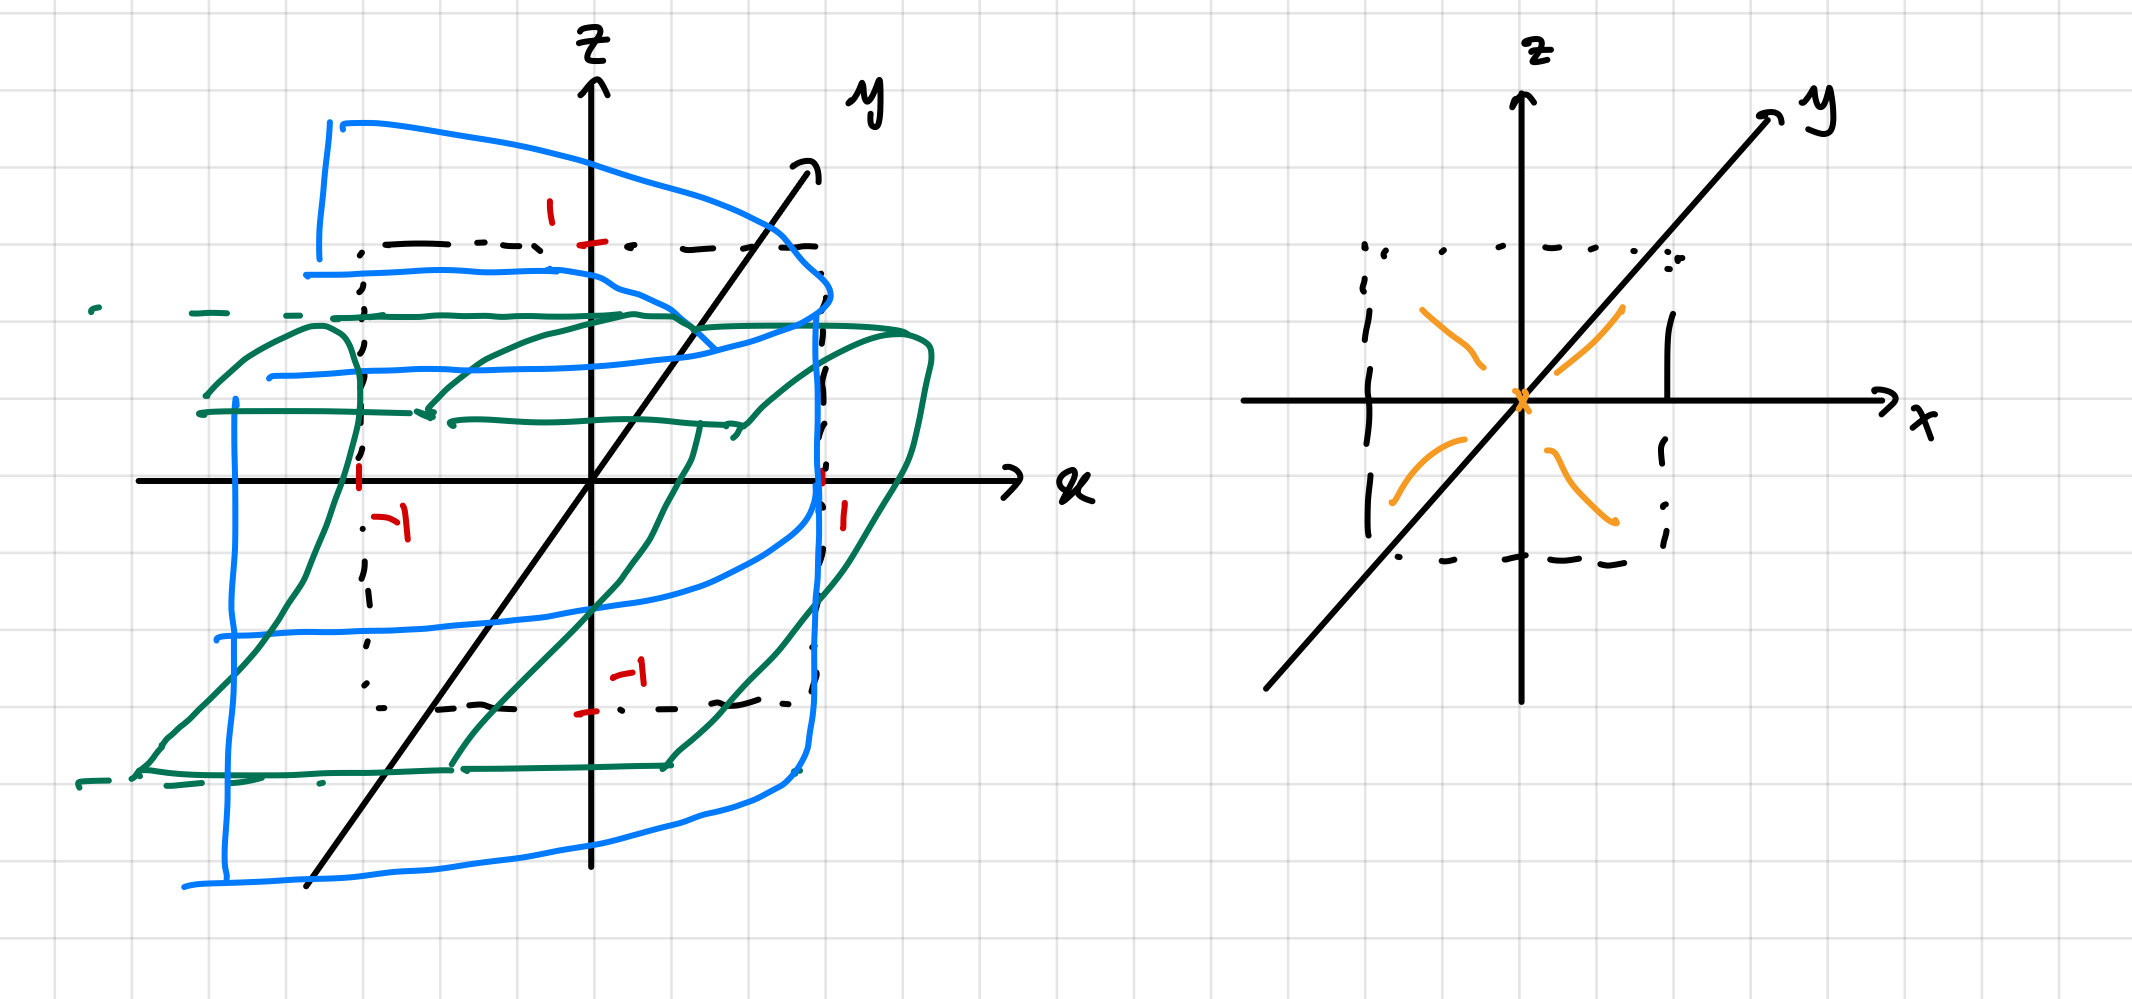
\includegraphics[width=13cm]{./figures/8.7b.jpeg}
    \end{center}
    The bounded volume is on the $[-1, 1] \times [-1, 1]$ square on the $xz-$plane, which consists of 4 identical volumes on each of the quadrant of the $xz-$plane. WLOG, consider the volume on the first quadrant, with $x, z \in [0, 1]$.
    Then for each $(x, z)$, $y_{min} = 1-1^2 = 0$, while \[
    y_{max} = \begin{cases}
    1-x^2 & \:\text{if}\: x \geq z \\
    1-z^2 & \:\text{if}\: x \leq z
    \end{cases}
    \]
    Taking volumes below and above the $z = x$ line, then the volume of this first-quadrant volume is
    \[
        V_1 = \abs*{\int_{0}^1 \int_{0}^{x} \int_{0}^{1-x^2}1 dy dz dx} + \abs*{ \int_{0}^{1} \int_{x}^{1} \int_{0}^{1-z^2} 1 dy dz dx}
    \]
    and the total volume throughout all 4 quadrants is just $4 V_1$.

    \textbf{(c)}
    \begin{align*}
    \int_{0}^{3} \int_{0}^{2} \int_{0}^{1} (2x + 3y^2 + 4z^3) dx dy dz &= \int_{0}^{3} \int_{0}^{2} \left[x^2 + 3y^2x + 4z^3x\right]_0^1 dy dz \\
    &= \int_{0}^{3} \int_{0}^{2} (1 + 3y^2 + 4z^3) \\
    &= \int_{0}^{3} \left[y + y^3 + 4z^3y\right]_0^2 dz \\
    &= \int_{0}^{3} (10 + 8z^3) dz \\
    &= 192
    \end{align*}
\end{solution}


\begin{problem} [VI \redtext{done}]
Let $\omega=\left(y \cos x y+\mathrm{e}^x\right) \mathrm{d} x+(x \cos x y+2 y) \mathrm{d} y$.
\begin{enumerate} [(a)]
    \item Evaluate $\int_{\Gamma} \omega$ along the segment of the parabola $y=x^2$ from $\begin{pmatrix}0 \\ 0\end{pmatrix}$ to $\begin{pmatrix}1 \\ 1\end{pmatrix}$. Use the parameterization $\phi: [0, 1] \to \R^2$
        \[
            \phi(t) = (t, t^2)
        \]
    \item  Evaluate $\int_{\Gamma} \omega$ for the case where $\Gamma$ is the straight line joining the origin to the point $\begin{pmatrix}\alpha \\ \beta\end{pmatrix}$. Do the same for the case where $\Gamma$ consists of the segment $0 \leqslant x \leqslant \alpha$ on the $x$-axis, followed by the segment $x=\alpha, 0 \leqslant y \leqslant \beta$.
    \item  Find a function $f(x, y)$  such that $\omega=d f$.
\end{enumerate}
\end{problem}
\begin{solution}
    \textbf{(a)} We get the pullback: \[
    \phi^* \omega = [(t^2 \cos (t^3) + e^t) + (t \cos (t^3) + 2t^2)(2t)]dt = (3t^2 \cos (t^3) + 4t^3 + e^t) dt
    \]
    Then \begin{align*}
    \int_{\Gamma} \omega &= \int_{0}^{1} (3t^2 \cos (t^3) + 4t^3 + e^t) dt \\
    &= \left[\sin(t^3) + t^4 + e^t\right]_0^1 \\
    &= \sin(1) + 1 + e - 1 = \sin(1) + e \qed
    \end{align*}

    \textbf{(b)} 
    \textbf{1.} Straight line joining origin to the point $\begin{pmatrix}
        \alpha \\
        \beta 
    \end{pmatrix}$
    is parameterized: \[
        \Gamma(t) = (\alpha t, \beta t)
    \]
    has pullback
    \begin{align*}
        \Gamma^* \omega &= [\alpha(\beta t \cos(\alpha \beta t^2) + e^{\alpha t}) + \beta(\alpha t \cos (\alpha \beta t^2) + 2 \beta t)] dt \\
        &= [2\alpha \beta t \cos (\alpha \beta t^2) + e^{\alpha t} + 2 \beta^2 t] dt
    \end{align*}
    so \begin{align*}
    \int_{\Gamma} \omega = \int_{0}^{1} \Gamma^* \omega &= \int_{0}^{1} [2\alpha \beta t \cos (\alpha \beta t^2) + \alpha e^{\alpha t} + 2 \beta^2 t] dt \\
    &= \sin(\alpha \beta) + e^\alpha - e + \beta^2
    \end{align*}

    \textbf{2.} Let $\rho$ parameterize path from $(0, 0)$ to $(\alpha, 0)$, and $\sigma$ parameterize path from $(\alpha, 0)$ to $(\alpha, \beta)$.
    \[
        \rho(t) = (\alpha t, 0), \sigma(t) = (\alpha, \beta t).
    \]
    They have pullback: \begin{align*}
    \rho^* \omega &= \alpha(e^{\alpha t}) dt \\
    \sigma^* \omega &= \beta (\alpha \cos(\alpha \beta t) + 2 \beta t) dt
    \end{align*}
    therefore \begin{align*}
    \int_{\Gamma} \omega &= \int_{\rho} \omega + \int_{\sigma} \omega \\
    &= \int_{0}^{1} (\alpha e^{\alpha t} + \alpha \beta \cos(\alpha \beta t) + 2\beta^2 t) dt \\
    &= \left[e^{\alpha t} + \sin(\alpha \beta t) + \beta^2 t^2\right]_0^1 \\
    &= e^\alpha - e + \sin(\alpha \beta) + \beta^2 \qed
    \end{align*}

    \textbf{(c)} \[
    f(x, y) = \sin xy + e^x + y^2
    \]
    has \begin{align*}
    \frac{\partial f}{\partial x} &= y \cos xy + e^x \\
    \frac{\partial f}{\partial y} &= x \cos xy + 2y
    \end{align*}
    so \[
    \omega = \frac{\partial f}{\partial x}dx + \frac{\partial f}{\partial y} dy = df
    \]
    as required.
\end{solution}

\begin{problem} [VII \redtext{done}]
Let $\omega=y \mathrm{~d} x-x \mathrm{~d} y$.

\begin{enumerate}
    \item[(a)] Evaluate $\int_\gamma \omega$ along the semicircle $\gamma$ from $\begin{pmatrix} r -1 \\ 0\end{pmatrix}$ to $\begin{pmatrix} r+1 \\ 0\end{pmatrix}$ defined by
        \[
            \begin{pmatrix}
                x \\
                y
            \end{pmatrix}=\begin{pmatrix}{r}
                -\cos t \\
                \sin t
            \end{pmatrix}
        \]
        for $0<t<\pi$.
    \item[(b)] Show explicitly that you can obtain a different value from that in (a) by choosing a different curve joining $\begin{pmatrix}{r}-1 \\ 0\end{pmatrix}$ to $\begin{pmatrix} r + 1 \\ 0\end{pmatrix}$.
\end{enumerate}
\end{problem}
\begin{solution}
    \textbf{(a)} With parameterization $\gamma(t) = (r - \cos t, \sin t)$ on $(0, \pi)$:
    \begin{align*}
    \int_{\gamma} \omega &= \int_{0}^\pi \sin^2 t - (r - \cos t) \cos t dt \\
    &= \int_{0}^{\pi} -r \cos t + 1 dt\\
    &= \left[-r \sin t + t\right]_0^\pi \\
    &= \pi
    \end{align*}

    \textbf{(b)} Parameterize $\rho(t) = (r - 1 + 2t, 0)$. Then $y = 0$ throughout and $dy = 0$. So $\int_{\rho} \omega = 0$, different from (a).
\end{solution}

\begin{problem} [VIII \redtext{done}]
In each of the following cases, $u$ and $v$ are functions on a plane where $x$ and $y$ are affine coordinates. Express $\mathrm{d} x \wedge \mathrm{d} y$ in terms of $\mathrm{d} u \wedge \mathrm{d} v$. Make a sketch showing typical curves $u=$ constant and $v=$ constant in the first quadrant $(x, y>0)$ and try to give a geometric interpretation to the relations between $\mathrm{d} x \wedge \mathrm{d} y$ and $\mathrm{d} u \wedge \mathrm{d} v$ by applying both to a parallelogram whose sides are tangent to $u=$ constant and $v=$ constant respectively.
\begin{enumerate}
    \item[(a)] $x=u \cos v . \quad y=u \sin v$.
    \item[(b)] $x=u \cosh v, \quad y=u \sinh v$.
    \item[(c)] $x=u^2-v^2, \quad y=2 u v$.
\end{enumerate}

\end{problem}
\begin{solution}
\mbox{}
    \begin{center}
        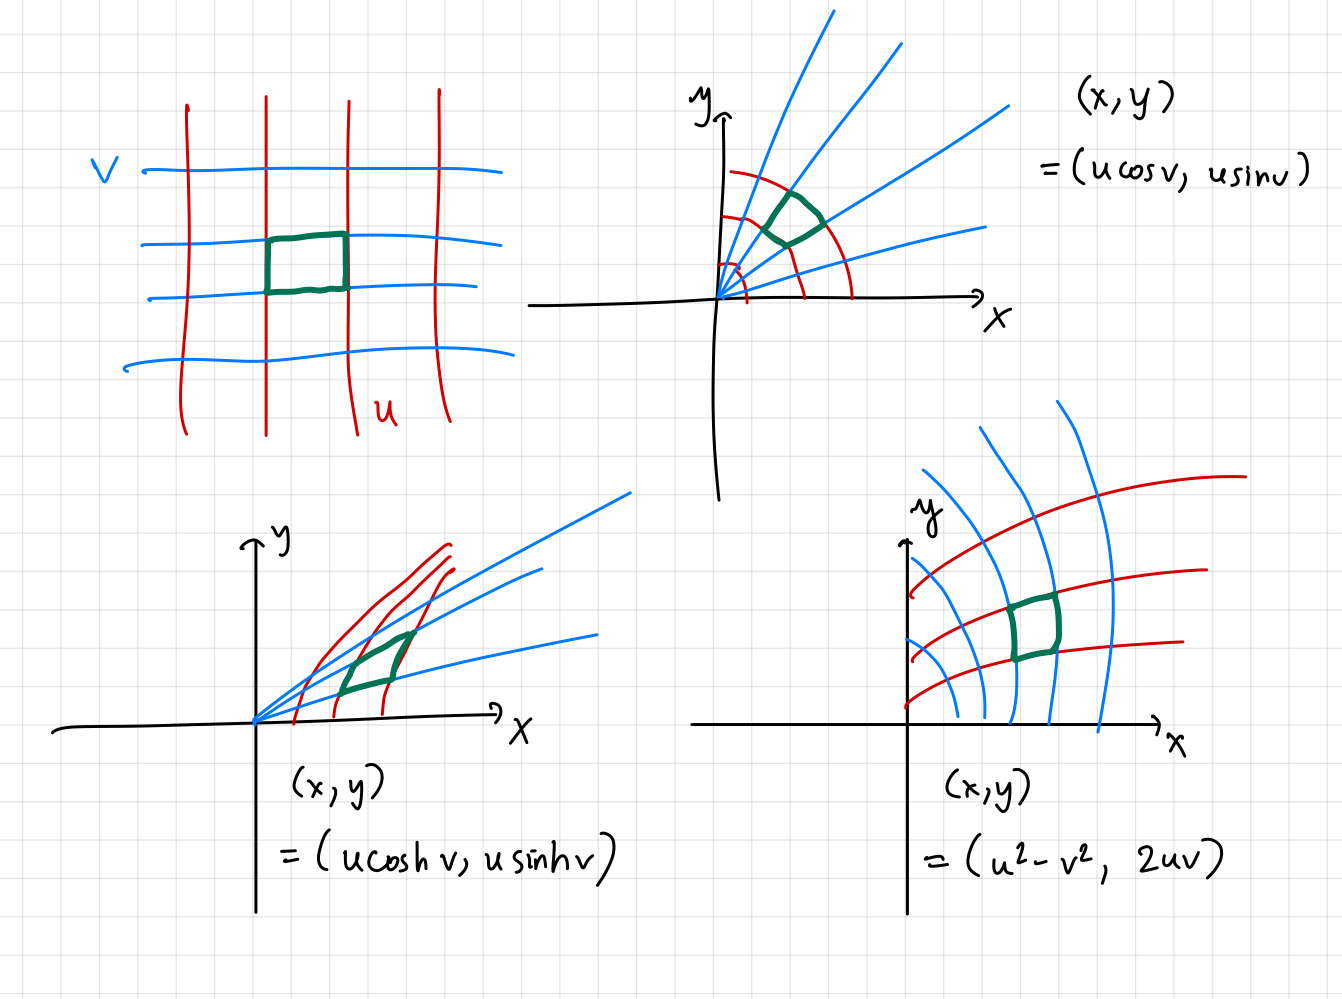
\includegraphics[width=15cm]{./figures/8.10.jpeg}
    \end{center}
    \textbf{(a)} \begin{align*}
        \rmd x &= \cos v \rmd u - u \sin v \rmd v \\
        \rmd y &= \sin v \rmd u + u \cos v \rmd v \\
        \implies \rmd x \wedge \rmd y &= u(\cos^2 v + \sin^2 v) \rmd u \wedge \rmd v \\
        &= u \rmd u \wedge \rmd v \\
    \end{align*}
    \textbf{(b)} \begin{align*}
    \rmd x &= \cosh v \rmd u + u \sinh v \rmd v \\
    \rmd y &= \sinh v \rmd u + u \cosh v \rmd v \\
    \implies \rmd x \wedge \rmd y &= u(\cosh^2 v - \sinh^2 v) \rmd u \wedge \rmd v \\
    &= u \rmd u \wedge \rmd v
    \end{align*}

    \textbf{(c)} \begin{align*}
    \rmd x &= 2u \rmd u - 2v \rmd v \\
    \rmd y &= 2v \rmd u + 2u \rmd v \\
    \implies \rmd x \wedge \rmd y &= (4u^2 + 4v^2) \rmd u \wedge \rmd v
    \end{align*}
\end{solution}

\begin{problem} [IX \redtext{done}]

\mbox{}
\begin{enumerate} [(a)]
    \item Show, by reversing the order of integration, that
        \[
            \int_0^a\left(\int_0^y \mathrm{e}^{m(a-x)} f(x) \mathrm{d} x\right) \mathrm{d} y=\int_0^a(a-x) \mathrm{e}^{m(a-x)} f(x) \mathrm{d} x
        \]
        where $a$ and $m$ are constants, $a>0$.
    \item Show that $\int_0^x\left(\int_0^v\left[\int_0^u f(t) \mathrm{d} t\right] \mathrm{d} u\right) \mathrm{d} v=\frac{1}{2} \int_0^x(x-t)^2 f(t) \mathrm{d} t$.
        If you do this in two steps, you never actually have to consider a triple integral!
\end{enumerate}
\end{problem}
\begin{solution}
    \textbf{(a)}
    \begin{align*}
        \int_0^a\left(\int_0^y e^{m(a-x)} f(x) dx\right) dy &= \int_{0}^{a} \int_{x}^{a} e^{m(a-x)} f(x) dy dx \\
        &= \int_{0}^{a} (a-x) e^{m(a-x)} f(x) dx
    \end{align*}
    as required.

    \textbf{(b)}
    \begin{align*}
        \int_0^x\left(\int_0^v\left[\int_0^u f(t) \mathrm{d} t\right] \mathrm{d} u\right) \mathrm{d} v &= \int_{0}^{x} \int_{0}^{v} \int_{t}^{v} f(t) \rmd u \rmd t \rmd v\\
        &= \int_{0}^{x} \int_{0}^{v} \left[u f(t)\right]_{u = t}^{u = v} \rmd t \rmd v\\
        &=\int_{0}^{x} \int_{0}^{v}(v-t)f(t) \rmd t \rmd v \\
        &= \int_{0}^{x} \int_{t}^{x} (v-t)f(t) \rmd v \rmd t \\
        &= \int_{0}^{x} \left[\frac{(v-t)^2}{2}\right]_{v = t}^{v = x} \rmd t \\
        &=\frac{1}{2} \int_0^x(x-t)^2 f(t) \mathrm{d} t
    \end{align*}
    as required.
\end{solution}

\end{document}